\documentclass{ximera}
%% Macros shared by every activity. Each activity loads this file with
%% %% Macros shared by every activity. Each activity loads this file with
%% %% Macros shared by every activity. Each activity loads this file with
%% \input{../preamble.tex}, and the xourse file with \input{preamble.tex}.

\newcommand{\RR}{\mathbb{R}}
\newcommand{\dfn}{\textit}
, and the xourse file with \input{preamble.tex}.

\newcommand{\RR}{\mathbb{R}}
\newcommand{\dfn}{\textit}
, and the xourse file with \input{preamble.tex}.

\newcommand{\RR}{\mathbb{R}}
\newcommand{\dfn}{\textit}


\title{Lines in the Plane}

\begin{document}
\begin{abstract}
Practice with slope, including a picture drawn with TikZ.
\end{abstract}
\maketitle

I like Taylor Swift.

\begin{image}
    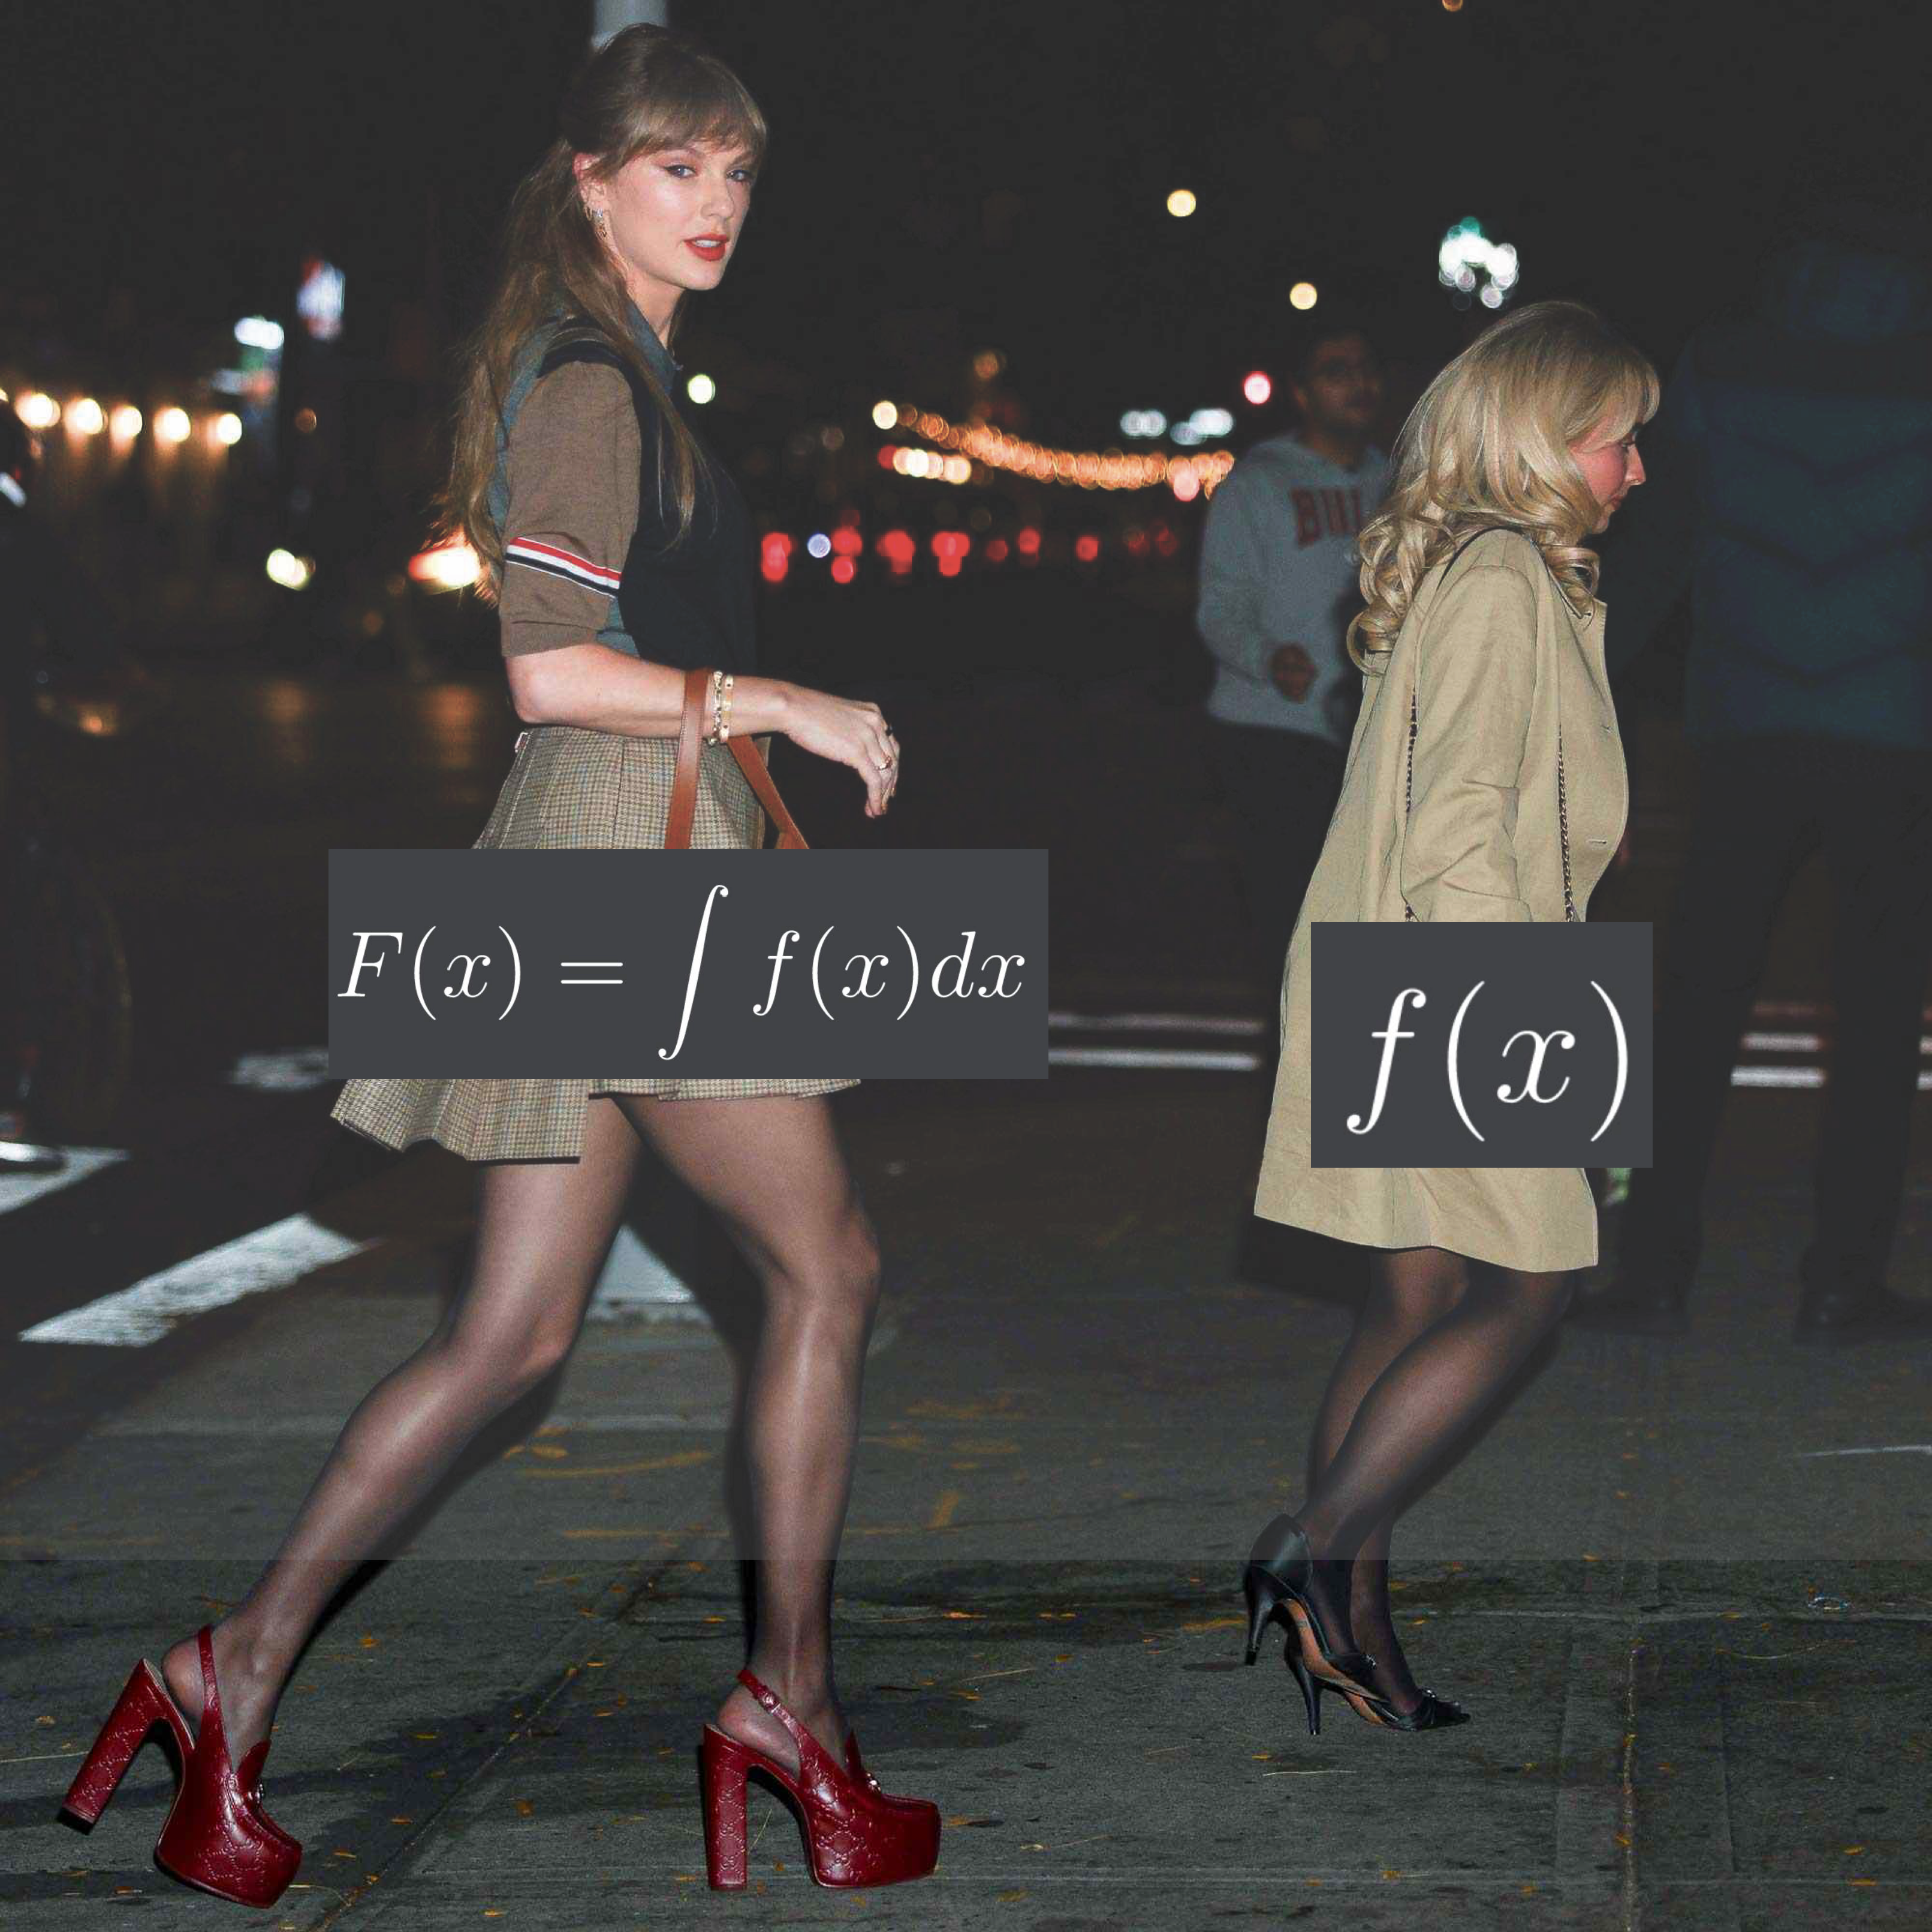
\includegraphics{src/lines/TS-Sabrina-Calc.png}
    \xmalt{Taylor Swift and Sabrina Carpenter photographed on a sidewalk. Taylor  is labeled with $F(x)=\int f(x)dx$ and Sabrina is labeled with $f(x)$. Taylor looks much taller than Sabrina.}
\end{image}

The \dfn{slope} of the line through two points is the change in $y$ divided
by the change in $x$.

\begin{problem}
The line below passes through the points $(1,1)$ and $(3,5)$.

\begin{center}
\begin{tikzpicture}[scale=.75]
  \draw[<->] (-1,0)--(5,0) node[right]{$x$};
  \draw[<->] (0,-1)--(0,6) node[above]{$y$};
  \draw[thick] (0.25,-0.5)--(3.5,6);
  \fill (1,1) circle (2pt) node[right]{$(1,1)$};
  \fill (3,5) circle (2pt) node[right]{$(3,5)$};
\end{tikzpicture}
\end{center}

Its slope is
\[
m=\answer{2}.
\]

Its equation in slope-intercept form is
\[
y=\answer{2}x+\answer{-1}.
\]
\end{problem}

\begin{problem}
A line perpendicular to the one above has slope
\[
m_{\perp}=\answer{-\frac{1}{2}}.
\]
\end{problem}

\end{document}
